%!TEX TS-program = xelatex

\documentclass {article}

\usepackage{xetexko}
\usepackage[a4paper]{geometry}
\usepackage[usenames,dvipsnames]{xcolor}
\usepackage{mathtools}
\usepackage{amsmath}
\usepackage{fontspec}
\usepackage{hyperref}
\usepackage{graphicx}
\usepackage{listings}
\usepackage{makeidx}
\usepackage{indentfirst}
\usepackage{tikz}
\usetikzlibrary{arrows,automata}


%\setmainfont {NanumMyeongjo}
\setmainfont {UnBatang}
\setmonofont[Scale=0.8]{DejaVu Sans Mono}

\lstdefinestyle{diff}{
  belowcaptionskip=1\baselineskip,
  breaklines=true,
  frame=L,
  xleftmargin=\parindent,
  showstringspaces=false,
  % Diffstart
  morecomment=[f][\color{gray}]{@@},
  % Diffincl
  morecomment=[f][\color{Green}]{+},
  % Diffrem
  morecomment=[f][\color{Red}]{-},
  basicstyle=\footnotesize\ttfamily,
}

\lstdefinestyle{customtxt}{
  belowcaptionskip=1\baselineskip,
  breaklines=true,
  frame=L,
  xleftmargin=\parindent,
  showstringspaces=false,
  basicstyle=\footnotesize\ttfamily,
}

\lstdefinestyle{customc}{
  belowcaptionskip=1\baselineskip,
  breaklines=true,
  frame=L,
  xleftmargin=\parindent,
  language=C,
  showstringspaces=false,
  basicstyle=\footnotesize\ttfamily,
  keywordstyle=\bfseries\color{green!40!black},
  commentstyle=\itshape\color{purple!40!black},
  identifierstyle=\color{blue},
  stringstyle=\color{orange},
}

\lstdefinestyle{customrs}{
  belowcaptionskip=1\baselineskip,
  breaklines=true,
  frame=L,
  xleftmargin=\parindent,
  showstringspaces=false,
  morekeywords={fn,let,mut,pub,use,impl,struct,unsafe,if,for},
  morecomment=[l]{//},
  morecomment=[n]{/*}{*/},
  basicstyle=\footnotesize\ttfamily,
  keywordstyle=\bfseries\color{green!40!black},
  commentstyle=\itshape\color{purple!40!black},
  identifierstyle=\color{blue},
  stringstyle=\color{orange},
}


\begin {document}

\title {AlgoSpot 문제 풀이}
\input {../../reportauthor.tex}
\maketitle

\section {Algospot 문제 - URI decoding}
\subsection {문제}
알고리즘 문제를 푸는 프로그래밍 대회에서, 문제 순서는 난이도와 관계가 없다. 이 문제는 앞에서부터 풀다가 뒤쪽에 있는 쉬운 문제를 놓치는 팀을 막기위해 출제되었다.

프로그래밍 대회에서 N개의 문제가 출제되었을 때, 난이도는 1이상 N이하인 자연수로 결정되고, 모든 문제는 서로 다른 난이도를 가진다. 또한, 숫자가 높을수록 어려운 문제를 의미한다. 그러므로 난이도 1이면 가장 쉬운 문제, N이면 가장 어려운 문제가 된다.

k번째로 쉬운 문제가 k번째에 배치되었다면, 이것을 "난이도 순으로 배치되었다."라고 한다. 역대 대회 문제들의 난이도가 입력으로 주어진다. 각 대회에 몇 문제가 난이도 순으로 배치되었는지 세어보자.

\subsection {입력}
알고리즘 문제를 푸는 프로그래밍 대회에서, 문제 순서는 난이도와 관계가 없다. 이 문제는 앞에서부터 풀다가 뒤쪽에 있는 쉬운 문제를 놓치는 팀을 막기위해 출제되었다.

프로그래밍 대회에서 N개의 문제가 출제되었을 때, 난이도는 1이상 N이하인 자연수로 결정되고, 모든 문제는 서로 다른 난이도를 가진다. 또한, 숫자가 높을수록 어려운 문제를 의미한다. 그러므로 난이도 1이면 가장 쉬운 문제, N이면 가장 어려운 문제가 된다.

k번째로 쉬운 문제가 k번째에 배치되었다면, 이것을 "난이도 순으로 배치되었다."라고 한다. 역대 대회 문제들의 난이도가 입력으로 주어진다. 각 대회에 몇 문제가 난이도 순으로 배치되었는지 세어보자.

\subsection {출력}
각 대회에 대해 난이도 순으로 배치된 문제의 개수를 출력한다.

\section {명세}
\subsection {개요}
이 프로그램은 주어진 수열을 정렬한 후, 정렬된 수열과, 주어진 수열에서 같은 위치에 있는 같은 수의 갯수를 세어 출력하는 프로그램이다.

\subsection {입력 정의}
프로그램에는 stdin 을 통해, $T \times 2 + 1$ 줄의 입력이 주어진다.

입력의 첫 줄 이후엔, 두 줄씩 프로그램이 변환해야 할 데이터가 주어진다.

입력의 줄은, <CR>, <LF>, <CR><LF> 와 같은 뉴라인 문자(열)을 통해 구분된다. - 문제에는 언급되지 않았으나, 추가됨.

입력의 첫째 줄은, 데이터 수열의 길이 $N$ 이고, 이는 $10 \le N \ge 12$ 를 만족한다.

입력의 둘째 줄은, 길이 $N$ 의 데이터 수열이고, 각 수는 공백 문자로 구분된다.

\subsection {출력 정의}
프로그램은 stdout 을 통해 입력을 받은 데이터를 가공한 것을 출력한다.

프로그램은 각 줄마다, 정렬된 수열과, 주어진 수열에서 같은 위치에 있는 같은 수의 갯수를 센 것을 출력한다.

출력의 줄 구분은 <LF> 뉴라인 문자를 이용해 구분한다.

출력의 순서는 입력된 데이터의 순서와 같다.

\subsection {종료 정의}
프로그램은, 변환 중에 위의 규칙으로 처리할 수 없는 경우를 발견할 경우,
exit status 에 적절한 오류 코드를 반환해야 한다.

만일 그렇지 아니할 경우, exit status 로 0 을 반환해야 한다.

\section {프로그램 설계}
\subsection {사용 언어}
프로그램을 Rust-lang 을 이용해 작성한다.
\subsection {구조}
Counter 클래스를 만들어, Counter 클래스가, 데이터 하나를 처리하는 형식으로 작성한다.
\subsection {해석 방식}
Counter 클래스가 생성될 때, 생성자로 해당 데이터 셋의 Vector를 받는다. 이후,
do\_count 함수가 호출되면, 주어진 Vector 를 정렬 후, 원래의 Vector 와 비교해서,
위치가 일치하는 수들을 센다.

\subsection {입력 방식}
stdin 을 개행 문자로 Tokenizing 하여 읽어주는 reader 객체를 사용,
첫 행에서, 테스트 조건의 길이를 읽고, 이후 두 줄씩 읽어서, 주어진 문자열을
Sanitizing 한 후, 벡터에 넣은 뒤, Counter 클래스로 객체를 생성 후 이를
Vector 에 넣는다..

\subsection {출력 방식}
Counter 객체가 들어있는 벡터를 이터레이션하며, do\_count 메서드를
호출해 반환된 값을 println! 을 이용, 한 줄에 한 개씩 출력한다.

\section {구현}
\lstinputlisting [style=customrs]{fix.rs}

\section {유닛 테스트}
유닛 테스트에서 테스트해야 할 것은, 주어진 프로그램이 스펙을 잘 준수하는지의
여부이다. 이를 위해, 구현상의 실수가 있을 수 있는 부분들을 예상해서 작성하게 된다.

이 문제에서는 다음과 같은 경우들을 생각해볼 수 있다.
\begin{itemize}
\item 주어진 데이터 셋의 길이보다, 실제로 주어진 데이터 셋의 길이가 미달한다면?
\item 주어진 데이터 셋의 길이보다, 실제로 주어진 데이터 셋의 길이가 초과한다면?
\item 데이터의 정렬이 잘 이루어 지는가?
\end{itemize}

첫째 경우의 데이터는,

3\newline
\indent3\newline
\indent1 2 3\newline

과 같은 입력과,

1\newline
\indent3\newline
\indent1 2\newline

와 같은 입력을 테스트 데이터로 생각해 볼 수 있으며,

두번째 경우에는,

1\newline
\indent3\newline
\indent1 2 3\newline
\indent3
\indent1 2 3\newline

혹은,

1\newline
\indent3\newline
\indent1 2 3 4\newline

을 생각해 볼 수 있다.

세번째 경우엔,

1\newline
\indent3\newline
\indent3 2 1\newline

과 같은 데이터를 넣어서, 프로그램이 결과로 1 을 반환하는지를 체크해 볼 수 있다.
\section {테스트}

\begin {figure}[h]
  \centering
  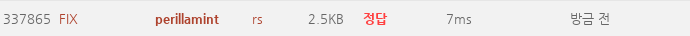
\includegraphics [width=120mm]{success.png}
  \caption {Success}
  \label{fig:Success}
\end {figure}

\end {document}
